\section{Obiettivo}
L'obiettivo di questo progetto è quello di realizzare un programma scritto in \textbf{OCaml} che risolva il \textit{problema} della \textit{colorazione di un grafo}: riuscire a colorare, se possibile, ogni nodo del grafo in modo da non avere mai nodi adiacenti con lo stesso colore. In via più formale, dato un grafo \lstinline[style=cmd]|g| ed un numero massimo di colori utilizzabili \lstinline[style=cmd]|N|, assegnare un colore ( da $0$ a $N-1$) ai nodi in modo tale che non esistano nodi adiacenti con lo stesso colore; qualora il numero di colori \lstinline[style=cmd]|N| non sia sufficiente per realizzare la colorazione, riportare un errore.
 
\section{Struttura del Progetto}

Di seguito sarà riportata la struttura delle cartelle e dei file del progetto con una breve descrizione per quelli più importanti. I file OCaml sono divisi in base al compito che svolgono le funzioni al loro interno (\textit{e.g.: \lstinline[style=cmd]|graphUtils| conterrà le funzioni che operano sui grafi, ecc.}) e sono sempre formati da un file \lstinline[style=cmd]|.ml| che contiene il copro delle funzioni con tutte le varie espressioni ed un file \lstinline[style=cmd]|.mli| nel quale è presente solo il tipo delle funzioni ed espressioni che verranno utilizzate dagli altri file.

\begin{figure}[H]
	\dirtree{%
		.1 .
		.1 Makefile.
		.1 src.
		.2 main.ml.
		.2 main.mli.
		.2 graphUtils.ml.
		.2 graphUtils.mli.
		.2 data.ml.
		.2 data.mli.
		.2 printer.ml.
		.2 printer.mli.
		.2 rappresentazione\_grafo.
		.3 rappresentazione\_grafo.py.
	}
	\caption{Rappresentazione schematizzata dei file e cartelle del progetto.}
\end{figure}

\begin{itemize}
	\item \lstinline[style=cmd]|Makefile|: utilizzato per compilare il progetto e generare l'eseguibile per avviarlo
	\item \lstinline[style=cmd]|main|: contiene la funzione principale che si occupa di avviare la colorazione e di gestire le scelte fatte dall'utente
	\item \lstinline[style=cmd]|graphUtils|: insieme di funzioni che operano sui grafi che svolgono l'effettivo compito di colorazione
	\item \lstinline[style=cmd]|data|: insieme di grafi per testare il corretto funzionamento del progetto. Questi possono essere aggiunti e rimossi in modo semplice ed efficiente
	\item \lstinline[style=cmd]|printer|: insieme di funzioni ed espressioni per stampare a video menu ed altri elementi con anche la presenza di colori ed emoji
	\item \lstinline[style=cmd]|rappresentazione_grafo|: script in python per rappresentare a video (in modo interattivo) un grafo
\end{itemize}
\ \\
Una volta utilizzato il comando \lstinline[style=cmd]|make| per compilare il progetto, la struttura finale delle cartelle sarà la seguente:

\begin{figure}[H]
	\dirtree{%
		.1 .
		.1 bin.
		.2 exe.
		.2 rappresentazione\_grafo.py.
		.1 build.
		.2 data.cmo.
		.2 graphUtils.cmo.
		.2 main.cmo.
		.2 printer.cmo.
		.1 Makefile.
		.1 src.
		.2 data.cmi.
		.2 data.ml.
		.2 data.mli.
		.2 graphUtils.cmi.
		.2 graphUtils.ml.
		.2 graphUtils.mli.
		.2 main.cmi.
		.2 main.ml.
		.2 main.mli.
		.2 printer.cmi.
		.2 printer.ml.
		.2 printer.mli.
		.2 rappresentazione\_grafo.
		.3 rappresentazione\_grafo.py.
	}
	\caption{Rappresentazione dei file e cartelle del progetto dopo averlo compilato.}
\end{figure}
\ \\
I file \lstinline[style=cmd]|.cmi| vengono lasciati all'interno della cartella \lstinline[style=cmd]|src| per far funzionare correttamente l'estensione di \textbf{OCaml} per \textbf{Visual Studio Code} e per la corretta compilazione degli altri file.

\section{Codice}
%TODO: spiegare prima come vengono rappresentati i colori (tipo il fatto che -1 vuol dire non colorato). E spiegare brevemente alcune funzioni importanti, non tutte ed in modo veloce e conciso.
\subsection{Rappresentazione di un Grafo}
In questo progetto i grafi (si parla sempre di grafi \textit{orientati/diretti}) vengono rappresentati come una \textit{tupla} di 3 elementi:

\begin{enumerate}
	\item \textbf{\lstinline[style=cmd]|succ|}: funzione successori che definisce tutti i successori (nodi vicini) di tutti i nodi del grafo
	\item \textbf{\lstinline[style=cmd]|start|}: nodo di partenza per la colorazione
	\item \textbf{\lstinline[style=cmd]|maxColors|}: numero massimo di colori da utilizzare durante la colorazione
\end{enumerate}
\ \\
Di seguito un esempio di definizione di un grafo con la sua rappresentazione: 
\begin{figure}[H]
	\begin{subfigure}[b]{.5\textwidth}
\begin{lstlisting}[style=caml]
let grafo_1 =
	let x = function        
		  0 -> [1; 2]
		| 1 -> [0; 2; 3]
		| 2 -> [0; 1]
		| 3 -> [1; 4]
		| 4 -> [3]
		| 5 -> [6]
		| _ -> [] in
	let start = 3 in
	let maxColors = 3 in
	let succ = Successori x in
	
	(Grafo (succ, start, maxColors))
;;
\end{lstlisting}
\caption{Esempio di definizione di un grafo}
	\end{subfigure}%
	\begin{subfigure}[b]{.5\textwidth}
			\centering
			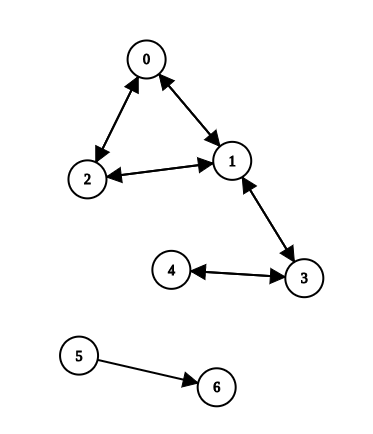
\includegraphics[width=.8\linewidth]{img/grafoesempio1.png}
			\caption{Grafo prodotto dal codice (a)}
	\end{subfigure}%
\end{figure}
\ \\
Il tipo \lstinline[style=cmd]|grafo| e \lstinline[style=cmd]|succesori|  sono definiti in \lstinline[style=cmd]|graphUtils| nel seguente modo:

\begin{lstlisting}[style=caml]
	type successori = Successori of (int -> int list);;
	type grafo 			= Grafo of successori * int * int;;
\end{lstlisting}
\newpage
\subsection{Data}
In questo file ci sono tutte le definizioni dei grafi utilizzati come test per verificare il corretto funzionamento dell'algoritmo di colorazione; una funzione che permette di stampare un menù, con alcune informazioni come la descrizione dei grafi e gli ID unici, ed una funzione che dato un numero (ID), ritorna uno dei grafi detti prima.
\`{E} anche presente una lista (\lstinline[style=cmd]|grafi|) che contiene tutti i grafi disponibili con una descrizione (una coppia \lstinline[style=cmd]|(grafo, string)|), è questa che permette di aggiungere e togliere elementi in maniera semplice e senza dover modificare alcuna funzione.\\

\begin{lstlisting}[style=caml, caption={Lista di coppie (grafo,string) utilizzata per assiocare ad un grafo una descrizione.}]
let grafi = [
	(grafo_1,   "Grafo 1"); 
	(grafo_2,   "Grafo 2 con numero sufficiente di colori"); 
	(grafo2err, "Grafo 2 con colori insufficienti"); 
	(grafo_3,   "Grafo 3"); 
	(grafo_4,   "Grafo 4")
];;
\end{lstlisting}

La funzione \lstinline[style=cmd]|stampa_grafi_disponibili| mostra a video la descrizione dei vari grafi anteceduta da un ID. Questa scandisce la lista \lstinline[style=cmd]|grafi| ricorsivamente e va a stampare il secondo elemento di ogni coppia.

\begin{figure}[H]
	\begin{subfigure}{\textwidth}

\begin{lstlisting}[style=caml]
let stampa_grafi_disponibili () = 
	let rec aux id = function (*lista di grafi*)
		  []      -> print_string "\n"    (*caso base, stampa un \n*)
		| x::coda ->                      (*stampa descrizione ed id*)
			let stampa_elemento (_, descrizione) = 
				print_string "  "; 
				print_int id; print_string (") " ^ descrizione ^ "\n")

			(*id + 1 e continua con la coda*)
			in  stampa_elemento x;    
				  aux (id+1) coda     

	in aux 1 grafi  (*avvia aux*)
;;
\end{lstlisting}
		\caption{Funzione per la stampa a video delle descrizione dei grafi antecedute da un ID}
	\end{subfigure}
\ \\
\ \\
	\begin{subfigure}{\textwidth}
		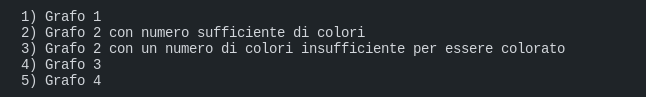
\includegraphics[width=\textwidth]{img/descrizione_grafi.png}
		\caption{Output del codice (a)}
	\end{subfigure}
\end{figure}

Infine, la funzione \lstinline[style=cmd]|scegli_grafo| che, dato un ID, ritorna il relativo grafo. \`{E} interessante notare come per selezionare un dato grafo non viene scorsa ricorsivamente tutta la lista, ma quest'utlima viene convertita in un \lstinline[style=cmd]|Array| per poter utilizzare il metodo \lstinline[style=cmd]|get| per accedere all'i-esima posizione. Vengono effettuati alcuni controlli sull'input: viene controllato se l'ID passato è valido (non superi per eccesso, o per difetto gli ID mostrati a video) e nel caso solleva un'eccezione (verrà utilizzata nella funzione \lstinline[style=cmd]|main| per segnalare il problema). %TODO: aggiungere riferimento

\begin{lstlisting}[style=caml, caption={Funzione che ritorna il grafo selezionato}]
let scegli_grafo id_grafo =
	let array_tmp = Array.of_list grafi in    (*lista in array*)
		if id_grafo > Array.length array_tmp || (*controlla id*)
		   id_grafo < 1  
			then 
				raise BadChoice    (* se non e valido lancia un'eccezione*)
		else
			fst (Array.get array_tmp (id_grafo-1))   (*ritorna grafo*)
;; 
\end{lstlisting}

\subsection{Printer}

In questo file risiedono tutte le funzioni e dichiarazioni che gestiscono la stampa a video. Vi è una definizione di stringhe per stampare su terminale caratteri colorati (rosso, verde, blu, ecc.),
elementi in grassetto ed emoji (a patto che quest'ultimo li supporti). La funzione più degna di nota è \lstinline[style=cmd]|stampa_grafo| che, dato un grafo, stampa a schermo tutti i nodi con i suoi vicini (in pratica rappresenta la funzione successori).\\
\ \\
Di seguito alcuni dei codici utilizzati per rappresentare i colori nel terminale: \\

\begin{lstlisting}[style=caml, caption={Codici per i colori ed elementi in grassetto}]
	type colore = Colore of string;;
	
	(* normali *)
	let rosso = Colore "\027[31m";;
	let verde = Colore "\027[32m";;
	let ciano =  Colore "\027[36m";;
	let bianco = Colore "\027[0m";;
	
	(* grassetto *)
	let rosso_b = Colore "\027[31;1m";;
	let verde_b = Colore "\027[32;1m";;
	let ciano_b = Colore "\027[36;1m";;
	let bianco_b = Colore "\027[0;1m";;
	
	(* valore di reset per stampare normalmente*)
	let reset = bianco;;
\end{lstlisting}

\begin{figure}[H]
\begin{subfigure}{\textwidth}
\begin{lstlisting}[style=caml]
let stampa_grafo (Grafo((Successori succ), partenza, maxColori)) =
	print_colore rosso_b "Partenza: ";
	print_int partenza; print_colore rosso_b " Max Colori: ";
	print_int maxColori; print_string "\n\n";
	let rec search visitati = function  (* frontiera *)
		  [] 				 -> print_string "\n"    (*caso base, stampa \n*)      
		| nodo::coda ->                      (*stampa nodo e vicini*)
			if List.mem nodo visitati     (* ignora nodi visti*)
				then 
					search visitati coda
			else                          (* stampa il nodo e vicini.*)
				(print_colore verde_b (string_of_int nodo); 
				print_colore bianco_b " -> "; stampa_lista (succ nodo); 
				search (visitati@[nodo]) (coda@(succ nodo)))

	in search [] [partenza]   (*avvia la ricorsione*)
;;
\end{lstlisting}
\caption{Funzione per la stampa di un grafo su terminale}
\end{subfigure}
\ \\
\ \\
\begin{subfigure}{\textwidth}
	\centering
	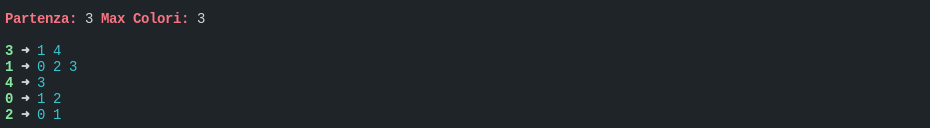
\includegraphics[width=\textwidth]{img/grafoTerminale.png}
	\caption{Output della funzione (a)}
\end{subfigure}
\end{figure}

\subsection{GraphUtils}

All'interno di questo file sono contenute tutte le funzioni e le espressioni che si occupano della gestione e  della colorazione dei grafi. In particolare, la funzione \lstinline[style=cmd]|colora| è quella che effettua la colorazione vera e propria. Prende in input un grafo (una tupla formata da \lstinline[style=cmd]|(successori, partenza, maxColori)|) e come output restituisce una lista composta da coppie del tipo \lstinline[style=cmd]|(nodo, colore)|, associa quindi ad ogni nodo (\lstinline[style=cmd]|int|) un colore (\lstinline[style=cmd]|int|). Alla riga \lstinline[style=cmd]|2| viene calcolato il \lstinline[style=cmd]|refValue| (servirà successivamente per cercare di trovare un possibile colore da assegnare qualora i vicini del nodo siano già stati colorati); nella riga \lstinline[style=cmd]|3| viene definita la funzione ausiliaria \lstinline[style=cmd]|esplora| che, tramite un algoritmo di ricerca in ampiezza (\textit{BFS}) andrà ad esplorare i nodi del grafo:

\begin{itemize}
	\item Se, il nodo esaminato è già stato visitato (è presente nella lista \lstinline[style=cmd]|visitati|) lo ignora e continua richiamando se stessa ed estraendo un nuovo nodo dalla frontiera (righe \lstinline[style=cmd]|7 - 9|)
	\item Altrimenti (il nodo non è mai stato analizzato), 
		\begin{itemize}
			\item aggiunge il nodo alla frontiera (lista di nodi da visitare),
			\item se possibile colora il nodo (aggiunge la coppia \lstinline[style=cmd]|(nodo, colore)| alla lista \lstinline[style=cmd]|colorati|), in caso contrario verrà sollevata un'eccezione, 
			\item infine aggiunge alla frontiera i nodi vicini al nodo esaminato. 
		\end{itemize}
	Richiama quindi se stessa con le nuove liste continuando così la ricorsione (righe \lstinline[style=cmd]|11 - 18|)
\end{itemize}
\ \\
Questa esplorazione avrà fine quando la frontiera non conterrà più nodi da esplorare.
La riga \lstinline[style=cmd]|20| serve per avviare la ricorsione (e quindi l'esplorazione) impostando le liste \lstinline[style=cmd]|vicini| e \lstinline[style=cmd]|colorati| come vuote e la frontiera con il nodo di partenza al suo interno. \\

\begin{lstlisting}[style=caml, caption={Funzione che si occupa della colorazione di un grafo.}, label=colora]
let colora (Grafo ((Successori succ), partenza, maxColori)) =
	refValue := calcola_refValue maxColori;   (*per colore mancante*)
	let rec esplora visitati colorati = 
		function (*frontiera*)
		 	  []            -> colorati  (*colorazione finita*)
			| nodo::coda    ->           (*continua a colorare*)
				if List.mem nodo visitati              (*nod visitato*)
					then 			(* ignora il nodo, successivo di frontiera*)
						esplora visitati colorati coda  

				else 	(*espande nodi vicini*)
					esplora 
						(visitati@[nodo])       (*nodo visitato*)
						(colorati@[
							(nodo, 
							(scegli_colore (Successori succ) nodo colorati maxColori)
							)]) (*colora il nodo*)
						(coda@(succ nodo))      (*aggiunge vicini a frontiera*)

	in esplora [] [] [partenza]   (*avvia esplora*)
;;
\end{lstlisting}
\ \\
Un'altra funzione molto importante all'interno di questo file è \lstinline[style=cmd]|scegli_colore|, che dati in input la \textit{funzione successori}, il \textit{nodo} da colorare, la lista dei \textit{nodi colorati} e il \textit{numero massimo di colori}, restituisce un colore (\lstinline[style=cmd]|int|) se possibile, altrimenti lancia un'eccezione (il numero di colori scelto è insufficiente per colorare il grafo). Alla riga \lstinline[style=cmd]|2, 7| viene scelto un potenziale risultato che è dato dal massimo tra i colori vicini al nodo aumentato di 1, in modulo \lstinline[style=cmd]|maxColori|. Così facendo ottengo una scelta ciclica dei colori, potendo ritornare a scegliere il colore 0 quando tutti gli altri sono stati assegnati.

\[
	risultato\_mod = (\max(colori\_vicini) + 1) \bmod maxColori
\]

\pagebreak
Quando un nodo non è stato colorato gli viene assegnato il valore \lstinline[style=cmd]|-1|, questo non inficia nel calcolo descritto prima: supponiamo di star analizzando il nodo iniziale, quindi sia lui che tutti i suoi vicini non hanno colore (colore = \lstinline[style=cmd]|-1|), il massimo risulterà essere \lstinline[style=cmd]|-1|. Il colore scelto sarà quindi \lstinline[style=cmd]|0| e verrà assegnato al nodo iniziale, tutto funziona come previsto.\\
\ \\
Infine viene analizzato questo possibile risultato (righe \lstinline[style=cmd]|8 - 16|):

\begin{itemize}
	\item Se il colore scelto è presente tra i colori dei nodi vicini (un nodo vicino ha già lo stesso colore), tenta di trovare un colore valido: somma tutti i colori vicini al nodo e sottrae questo valore al \lstinline[style=cmd]|refValue|. Se questo nuovo colore è ancora uguale ad un colore vicino al nodo, viene lanciata un'eccezione dato che non è possibile risolvere il problema, altrimenti viene ritornato come nuovo colore (righe \lstinline[style=cmd]|8 - 15|).
	\item Se non lo è allora vuol dire che è stato scelto il giusto colore e viene ritornato.
\end{itemize}

In questo modo, mi assicuro che ad ogni passaggio viene scelto il colore giusto e non necessito di dover ricontrollare tutto il grafo nuovamente.\\

\begin{lstlisting}[style=caml, caption={Funzione ausiliaria a \autoref{colora} che sceglie un colore per il nodo (se possibile).}]
	let scegli_colore (Successori succ) nodo colorati maxColori = 
		let risultato = 	(*trova il massimo tra i colori vicin al nodo +1*)
			((max_colore_vicini (Successori succ) nodo colorati)+1) in
		
		(*trova tutti i colri vicini*)
		let colori_vicini = tutti_colori_vicini (succ nodo) colorati in            
		let risultato_mod = risultato mod maxColori in  (*calcola il modulo*)
			if List.mem risultato_mod colori_vicini  
				then 	 (*colore scelto = colore vicino*)
					let mancante = 	(* prova scegliere un altro colore*)
						trova_mancante colori_vicini maxColori in     
							if List.mem mancante colori_vicini 
								(* numero di colori insufficiente *)
								then raise InsufficentColorNumber                             
							else mancante	(*ritorna colore mancante*)
			else risultato_mod	(*trovato un colore valido*)
;;
\end{lstlisting}
%TODO: cercare di aggiungere un esempio di come funziona questo calcolo

Infine un breve sguardo alla funzione che si occupa di salvare i dati del grafo colorato su file per poterli poi processare da python e mostrare una versione interattiva del grafo a video. Viene scandita tutta la lista prodotta dalla funzione \autoref{colora} (lista di coppie \lstinline[style=cmd]|(nodo, colore)|) e per ogni elemento viene scritto  su file: 

\begin{center}
	\lstinline[style=cmd]|nodo,vicini,colore|
\end{center}

Un esempio: \lstinline[style=cmd]|0,1 2 9 3,1|. Questo vuol dire che il nodo \lstinline[style=cmd]|0| ha come vicini \lstinline[style=cmd]|1, 2, 9, 3| e come colore \lstinline[style=cmd]|1|. Nelle righe \lstinline[style=cmd]|4 - 10| viene definita una funzione ausiliaria che permette di salvare la lista dei nodi adiacenti e la parte di codice che effettua le operazioni descritte prima è nelle righe \lstinline[style=cmd]|12 - 21|.

\begin{lstlisting}[style=caml, caption={Funzione che salva un grafo su file.}]
let grafodati_file = "grafo.data";; (*file dove salvare il grafo*)
let salva_grafo_colorato (Successori succ) colorati = 
	let oc = open_out grafodati_file in	(*apertura file in scrittura*)
		let rec salva_lista =   (*salva su file una lista*)
			function (* lista *)
				 [x]      -> Printf.fprintf oc "%d" x   (* caso base*)
				| _ 		  -> ()
				| x::coda ->                            (* caso ricorsivo*)            
					Printf.fprintf oc "%d " x;         (* stampa l'elemento*)
					salva_lista coda                   (* continua*)
				
		in let rec salva =      (*salva nodo - vicini - colore su file*)
			function (* lista nodi_colorati *)
				 []  -> 
				 	Printf.fprintf oc "\n"; 
				 	close_out oc  (*chiude file*)
				|(nodo, colore)::coda -> (* salva nodo,vicini,colore*)
					Printf.fprintf oc "%d," nodo; 
					salva_lista (succ nodo); Printf.fprintf oc ","; 
					Printf.fprintf oc "%d\n" colore; 
					salva coda	(*continua*)

	in salva colorati (*avvia salva*)
;;
\end{lstlisting}


\subsection{Main}

In questo file è presente la funzione principale \lstinline[style=cmd]|main| che si occupa di gestire tutto il flusso del programma: stampa il menu iniziale, fa scegliere all'utente su quale grafo testare l'algoritmo di colorazione, avvia la colorazione del grafo selezionato, stampa il risultato ed avvia lo script python.
\newpage
\begin{lstlisting}[style=caml, caption={Parte del codice contenuto in main.ml }]
let main () = 
	stampa_logo ();                 (*stampa il logo*)
	stampa_grafi_disponibili ();    (*stampa i grafi disponibili*)

	let dati = 
		let rec aux () =               (*utente sceglie il grafo*)
			try                          (*controllo input valido*)
				scegli_grafo (scelta ())
			with BadChoice -> 
				aux () 
		in aux() 
			in let avvia_colorazione (Grafo (g, partenza, maxColori)) = 
				print_string "\nIl Grafo selezionato: \n\n"; 
				stampa_grafo (Grafo (g, partenza, maxColori)); 
				print_string "Coloro ...\n\n";
				 
				(*colora il grfo*)
				let colorati = colora (Grafo (g, partenza, maxColori)) in     
					stampa_nodi_colorati colorati;   (*stampa il grafo colorato*)
					salva_grafo_colorato g colorati; (*salva grafo colorato*)
					avvia_python ()                  (* avvia python*)

					in      (*con un grafo scelto, lo colora*)
						try                                
							avvia_colorazione dati  
						with InsufficentColorNumber -> 
							stampa_errore ()
;;

\end{lstlisting}
\ \\
Alla riga \lstinline[style=cmd]|2 - 3| viene stampato sul terminale il logo iniziale e tutti i grafi disponibili per testare l'algoritmo. Nelle successive righe (\lstinline[style=cmd]|5 - 27|) vengono definite alcune funzioni ausiliarie per mettere in pratica i comportamenti descritti prima:

\begin{itemize}
	\item \lstinline[style=cmd]|dati|: rimane fermo sulla scelta del grafo fin quando l'utente non seleziona un ID esistente. Una volta selezionato un ID valido conterrà il grafo scelto. %TODO: scrivere meglio
	\item \lstinline[style=cmd]|avvia_colorazione|: stampa alcune informazioni utili all'utente per poi colorare il grafo, salvarlo su file e avviare lo script python. Qui vengono anche gestite le possibili eccezioni.
\end{itemize}
\ \\
Nelle prime righe del file vengono inclusi gli altri codici descritti prima con:

\begin{lstlisting}[style=caml, caption={Inclusione degli altri file .ml}]
 open Printer;;
 open GraphUtils;;
 open Data;;
\end{lstlisting}
\subsection{Python}

All'interno del progetto è anche presente un breve script in python che verrà avviato una volta riuscito a colorare il grafo. Questo script legge il file \lstinline[style=cmd]|.data| generato da OCaml (contiene il grafo ed i colori di ogni nodo) e lo rappresenta all’interno di una finestra in modo interattivo e soprattutto più comprensibile rispetto alla visualizzazione su terminale.\\

\begin{lstlisting}[style=python, caption={Alcune funzioni dello script python}]
from pyvis.network import Network


def main(fname):
	collegamenti = []
	nodi = []
	colori = []

	# lettura dei dati da file
	with open(fname, 'r') as f:
		for text in f.readlines():
		text = text.strip("\n")               # elimina i vari \n nel file
		if text != '':                        # controlla validita' riga
			nodo, vicini, colore  = text.split(",")

			vicini = vicini.split(" ")  			 # prende i vicini
			colori.append(int(colore))         # aggiunge il colore alla lista

			if vicini[0] != '':                # controlla se il nodo ha vicini
				for vicino in vicini:            # crea gli archi del grafo
					tmp = (int(nodo), int(vicino))
					collegamenti.append(tmp)    

	nodi = trova_nodi(collegamenti) 
	colori = aggiusta_colori(colori)  # converte i colori per pyvis
	
	# rappresenta il grafo con pyvis
	rappresenta_grafo(nodi, collegamenti, colori) 
 
 
 def rappresenta_grafo (nodi, collegamenti, colori):
	net = Network(width='100%', height='600px', directed=False)
 
 	net.add_nodes(nodi, color=colori)
 	net.add_edges(collegamenti)
 	net.toggle_physics(True)
 	net.inherit_edge_colors(False)
 
 	net.show('rappresentazione_grafo.html')
   		
\end{lstlisting}

\begin{figure}[H]
	\centering
	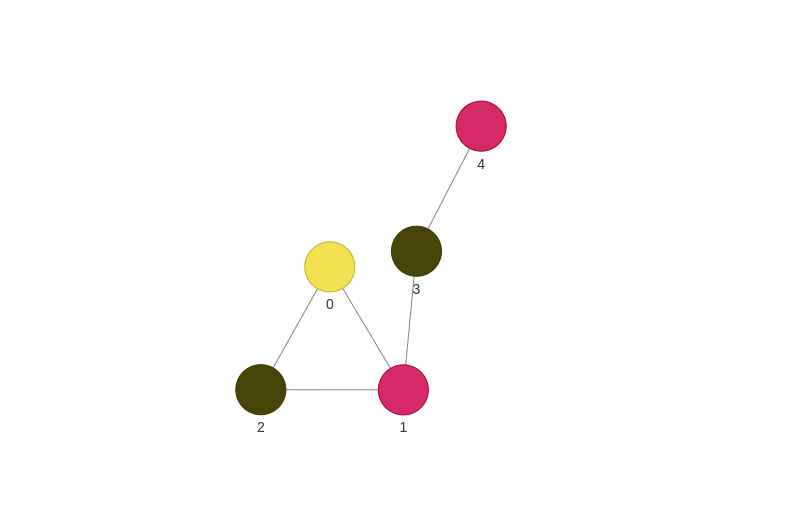
\includegraphics[width=.6\textwidth]{img/grafocoloratopy.png}
	\caption{Output dello script python.}
\end{figure}

\subsection{Makefile}

File utilizzato per la compilazione del progetto che avviene tramite il comando \lstinline[style=cmd]|make|. 
Qualora un file venga modificato, questo permette di non dover ricompilare tutto il progetto ma solo quello che è stato cambiato. In una prima fase compila tutti i file \lstinline[style=cmd]|.ml| con i relativi \lstinline[style=cmd]|.mli|, generando 2 altri file:

\begin{itemize}
	\item \lstinline[style=cmd]|.cmi|: interfacce compilate utili per il corretto funzionamento dell'estensione \textit{OCaml} in \textit{Visual Studio Code} e per la corretta compilazione degli altri file.
	\item \lstinline[style=cmd]|.cmo|: file oggetto che verranno poi spostati nella cartella \lstinline[style=cmd]|build| per essere utilizzati nella fase di \textit{linking}
\end{itemize}

Quindi, ogni file \lstinline[style=cmd]|.cmo| dipende dai relativi file \lstinline[style=cmd]|.ml| e \lstinline[style=cmd]|.mli|.
Successivamente, avvia la fase di \textit{linking} unendo insieme tutti i file \lstinline[style=cmd]|.cmo| e generando l'eseguibile \lstinline[style=cmd]|exe| nella cartella \lstinline[style=cmd]|bin|. All’interno di quest’ultima viene copiato anche lo script python per permettere il corretto funzionamento del progetto.\\

\begin{lstlisting}[style=make, caption={Breve estratto del file Makefile}]
cc = ocamlc
cflags = -c
cinclude = -I src
srcdir = src
buildir = build
bindir = bin
target = $(bindir)/exe

.PHONY: clear
all: cartelle $(target)

$(target): 
	$(buildir)/graphUtils.cmo $(buildir)/printer.cmo 
	$(buildir)/data.cmo $(buildir)/main.cmo
		$(cc) -o $@ $^
		cp $(srcdir)/rappresentazione_grafo/rappresentazione_grafo.py $(bindir)

\end{lstlisting}

\section{Dimostrazione}

Di seguito andremo a vedere una breve guida dimostrativa del funzionamento del progetto, dalla compilazione iniziale fino al grafo colorato.

\subsection{Compilazione}
Per prima cosa è necessario compilare il progetto. Bisogna spostarsi all'interno della cartella \lstinline[style=cmd]|progetto|, dove è contenuto il file \lstinline[style=cmd]|Makefile| e la cartella \lstinline[style=cmd]|src|. Ora avviare la compilazione con il comando:

\begin{center}
	\lstinline[style=cmd]|make|
\end{center}
\ \\
Verranno create due nuove cartelle: 

\begin{itemize}
	\item \lstinline[style=cmd]|bin|: al suo interno ci sarà l'eseguibile \lstinline[style=cmd]|exe| ed altri file necessari al funzionamento del progetto
	\item \lstinline[style=cmd]|build|: conterrà tutti i file generati durante la fase di compilazione (\lstinline[style=cmd]|.cmo|)
\end{itemize}

\begin{figure}[H]
	\centering
	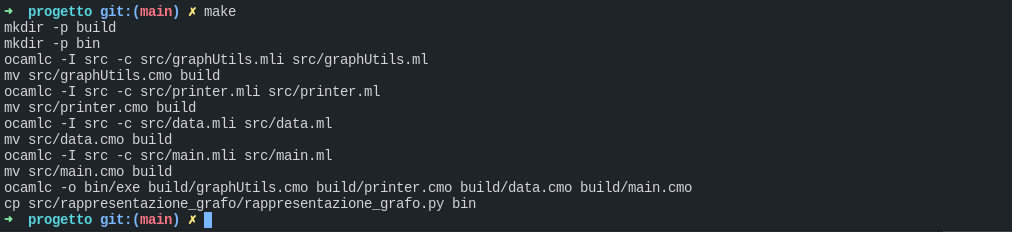
\includegraphics[width=\textwidth]{img/make.png}
	\caption{Output del comando make}
\end{figure}

Qualora si voglia ripulire tutti i file generati da questa operazione è possibile tramite il comando:

\begin{center}
	\lstinline[style=cmd]|make clear|
\end{center}
\ \\
\begin{figure}[H]
	\centering
	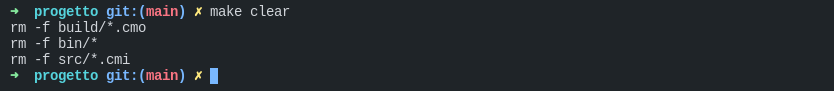
\includegraphics[width=.8\textwidth]{img/makeclear.png}
	\caption{Output del comando make clear}
\end{figure}

\subsection{Esecuzione}

Per avviare l'eseguibile del progetto generato alla fase precedente è prima necessario spostarsi all'interno della cartella \lstinline[style=cmd]|bin|:

\begin{center}
	\lstinline[style=cmd]|cd bin|\\
	\lstinline[style=cmd]|./exe  |
\end{center}

Verrà mostrato il menù iniziale e l'utente dovrà scegliere quale grafo utilizzare per testare l'algoritmo di colorazione.

\begin{figure}[H]
	\centering
	
\includegraphics[width=.8\textwidth]{img/menu.png}
	\caption{Menu iniziale}
\end{figure}

Se viene inserito un ID invalido, si rimane bloccati in questa scelta fin quando un ID esistente non viene inserito.

\begin{figure}[H]
	\centering
	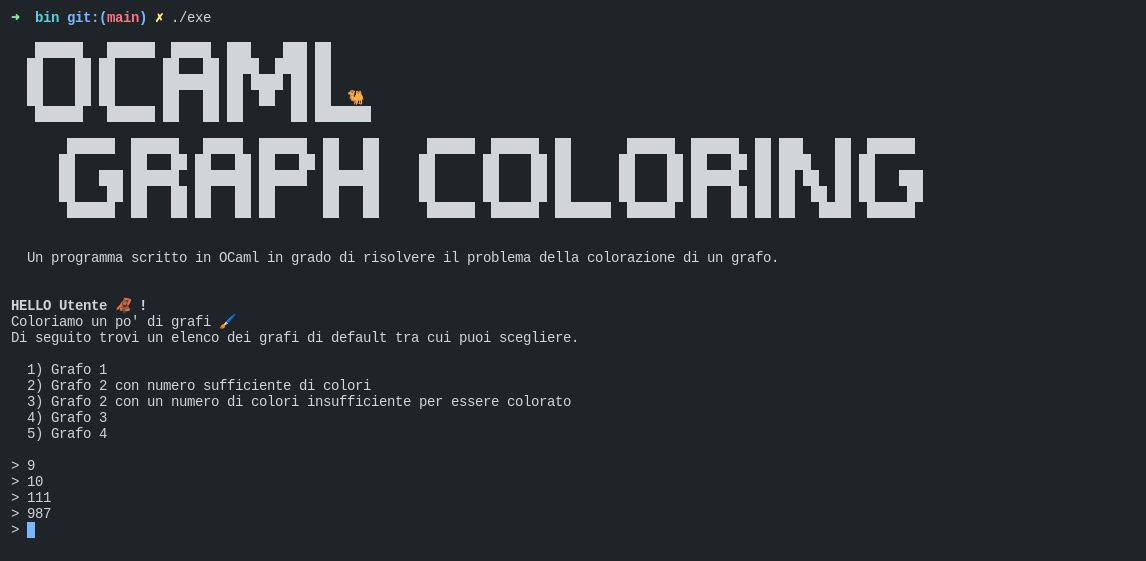
\includegraphics[width=.8\textwidth]{img/badid.png}
	\caption{Esempio di multipli ID errati}
\end{figure}
\ \\
Una volta selezionato un ID valido verrà stampato a video il grafo, con il nodo di partenza, il massimo numero di colori ed il risultato della fase di colorazione.

\begin{figure}[H]
	\centering
	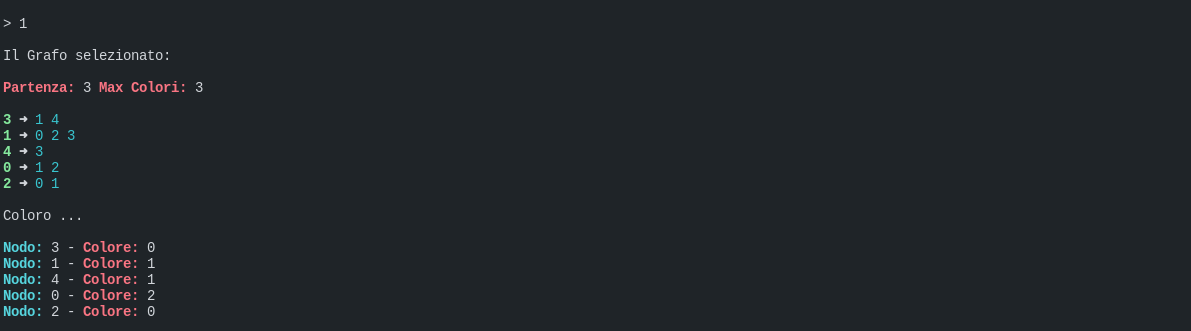
\includegraphics[width=.8\textwidth]{img/grafo1bin.png}
	\caption{Esempio di colorazione di un grafo}
\end{figure}

Infine verrà avviato lo script python che aprirà una finestra con al suo interno il grafo disegnato.

\begin{figure}[H]
	\centering
	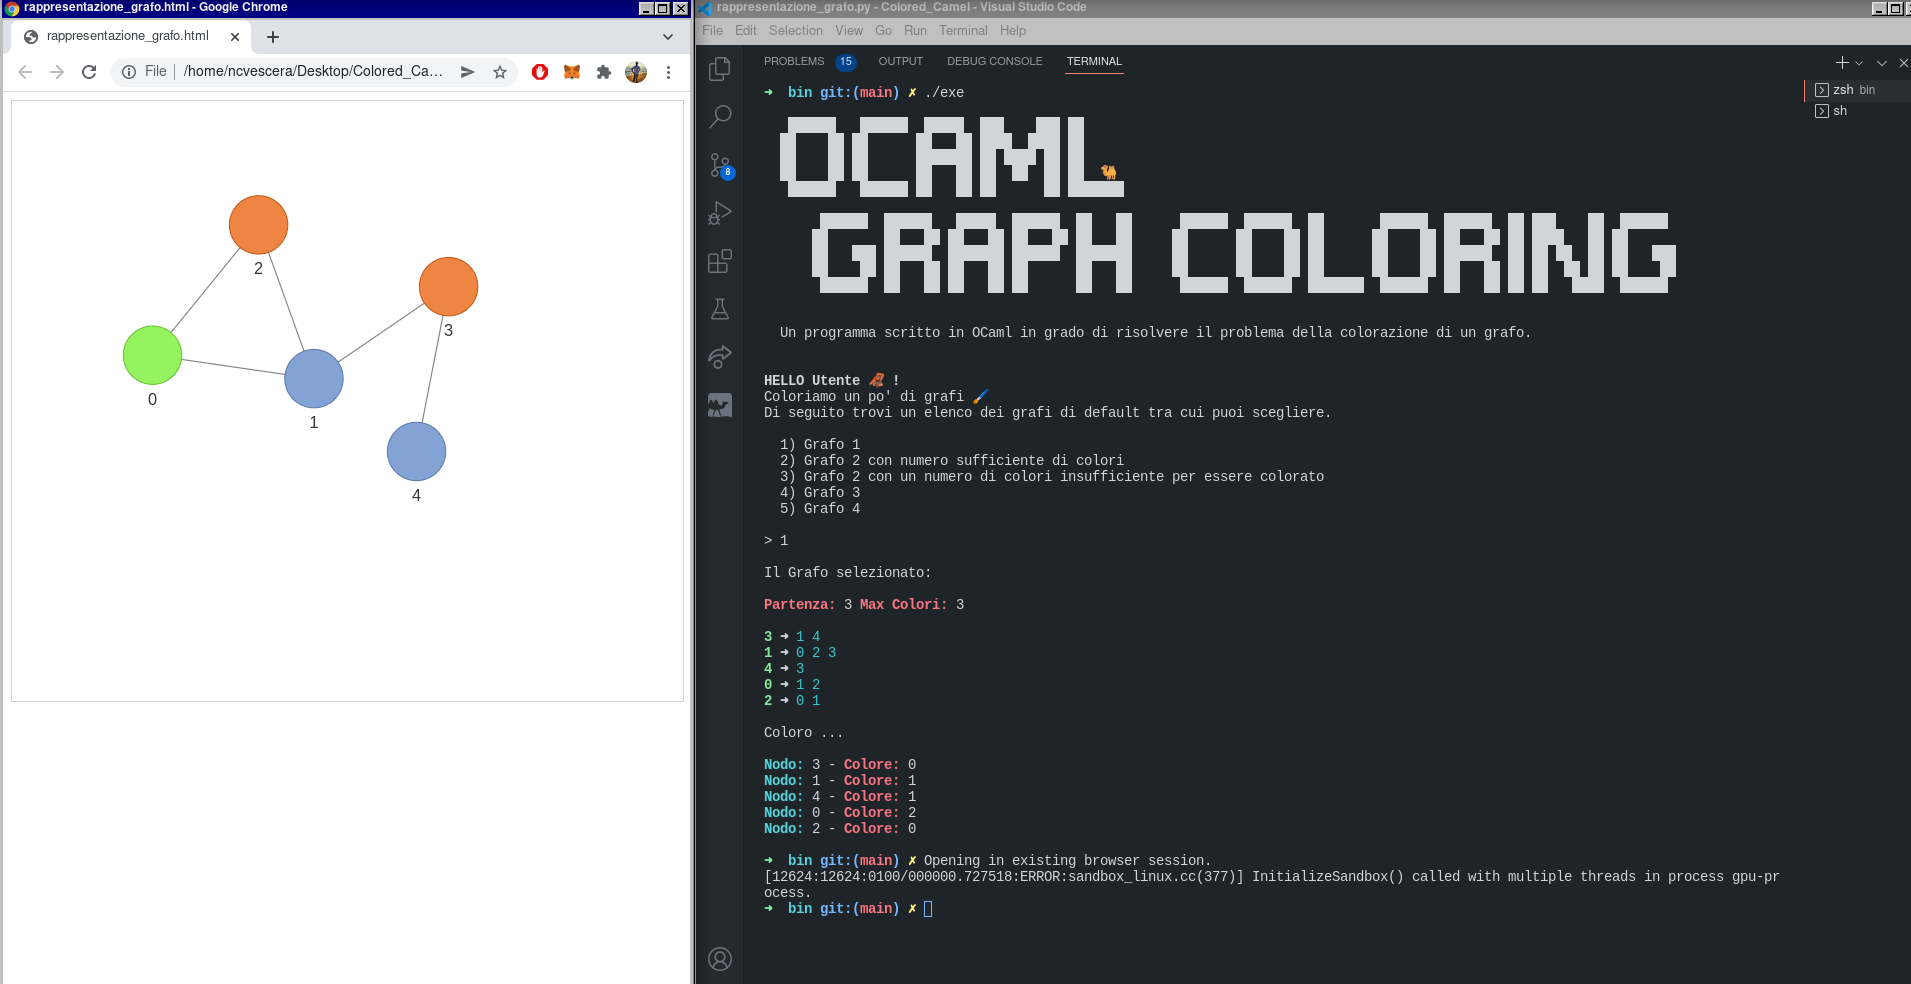
\includegraphics[width=.7\textwidth]{img/termgrafo.png}
	\caption{Finestra aperta da python con terminale affiancato}
\end{figure}

Qualora l'utente selezionerà un grafo che non è colorabile per via del numero insufficiente di colori, verrà mostrato a video un messaggio di errore e non verrà avviato lo script python.

\begin{figure}[H]
	\centering
	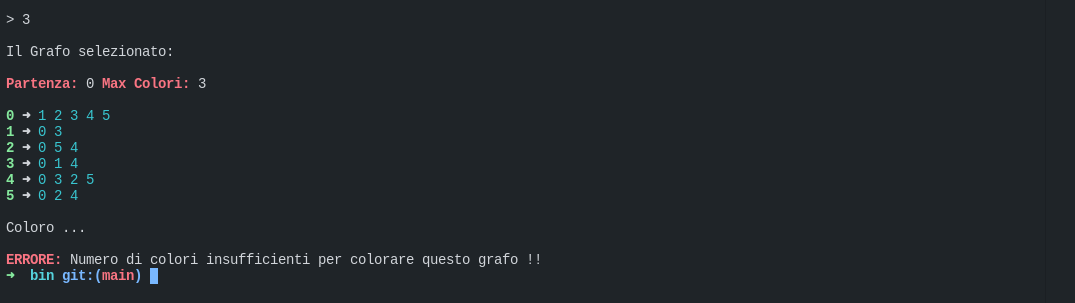
\includegraphics[width=.7\textwidth]{img/errore.png}
	\caption{Messaggio di errore per numero di colori insufficienti}
\end{figure}